The components that make up OpenDTrace interact with each other to
implement an operational model for dynamic tracing.  At the highest
level there are three components to OpenDTrace: tools, such as
\texttt{ctfconvert} which take compiled object code and generate new
ELF/DWARF sections that capture type information, the kernel module,
which is responsible for adding and removing trace points at run time,
and the libraries, which tie all of the components together.  Users
interact with OpenDTrace via the \texttt{dtrace} command line tool.

The OpenDTrace kernel module is the heart of the DTrace
framework. This module is responsible for the coordination of all
other components used in instrumentation. It keeps track of all
registered providers and informs them when to enable or disable their
probes. When a probe fires, the OpenDTrace kernel module is
responsible for executing the necessary instrumentation code and
providing the data to any consumers.

The kernel module is also the intermediary between the DTrace user
interface and the providers. When compiling user scripts, the kernel
module provides the D compiler with probe arguments and types. Once
compiled, scripts are pushed into the kernel as Enabling Control Blocks
(ECBs) to be executed when probes fire. After each ECB is executed,
the data is handed back to user space where the \texttt{dtrace}
command line tool, or other programs linked against the OpenDTrace
libraries can manipulate or display the data to end users.

Providers in OpenDTrace encapsulate the probe points that are used to
instrument code and provide data to the end user. A provider defines
both a set of probe points as well as the standard by which the system
interacts with that set of probe points.  For example, the Function
Boundary Tracepoint (\texttt{fbt}) provider, not only gives D scripts
access to function entry points and their arguments, but also access
to the return from a function.  The \texttt{fbt} provider, following
the C ABI standard, defines a \texttt{return} trace point to have only
two arguments: zero ($0$) and one ($1$).  The zero'th argument to any
\texttt{return} probe always contains the return value and the first
argument contains return address.  The \texttt{return} probe is
specific to the \texttt{fbt} provider, and no other provider has such
a definition.

OpenDTrace has a base set of providers that are shipped as part of the
system, see Appendix~\ref{chap:opendtrace-providers}, but developers are free to
create their own, to expose more or different information from their
code. Providers can be developed either for the kernel, in which case
they are defined as kernel modules, or for user space, as part of the
Userland Statically Defined Tracing (USDT) system.

A provider is simply a collection of probe points. Probe points are
functions that are run when certain points in the code are
reached. The probe gathers data of interest and passes data back into
the OpenDTrace kernel module for further processing. Since the
overhead of probes should be avoided when data is not required, the
provider is responsible for tracking when probes are enabled and
implementing a mechanism for the kernel module to update their state.

The user space interface to OpenDTrace is the \texttt{drace(1)}
command line utility. The \texttt{dtrace} command line utility handles
all run time interaction with the OpenDTrace system, such as
submitting scripts for execution as well as configuring options as
memory usage, and how often the system should flush data from the
kernel.  The complete syntax and set of options for the
\texttt{dtrace} command is given in the \texttt{dtrace(1)} manual
page.

The majority of the DTrace CLI functionality is provided through calls
to the DTrace user-space library, \texttt{libdtrace}, which is
responsible for setting DTrace options, compiling D scripts, and
passing compiled D code to the kernel for
execution. \texttt{libdtrace} provides the mechanism for all
interactions with DTrace in the kernel.

\section{Probe Life Cycle}
\label{sec:lifecycle}

An example of instrumentation with OpenDTrace is shown in
Figure~\ref{fig:lifecycle}. We assume that the OpenDTrace kernel
module has already been loaded during system boot. We ignore the
execution of code within any of the providers and only discuss the
interactions between components. Internal functions of interest within
the kernel module and CLI are shown.

\begin{figure}[htpb]
	\centering
	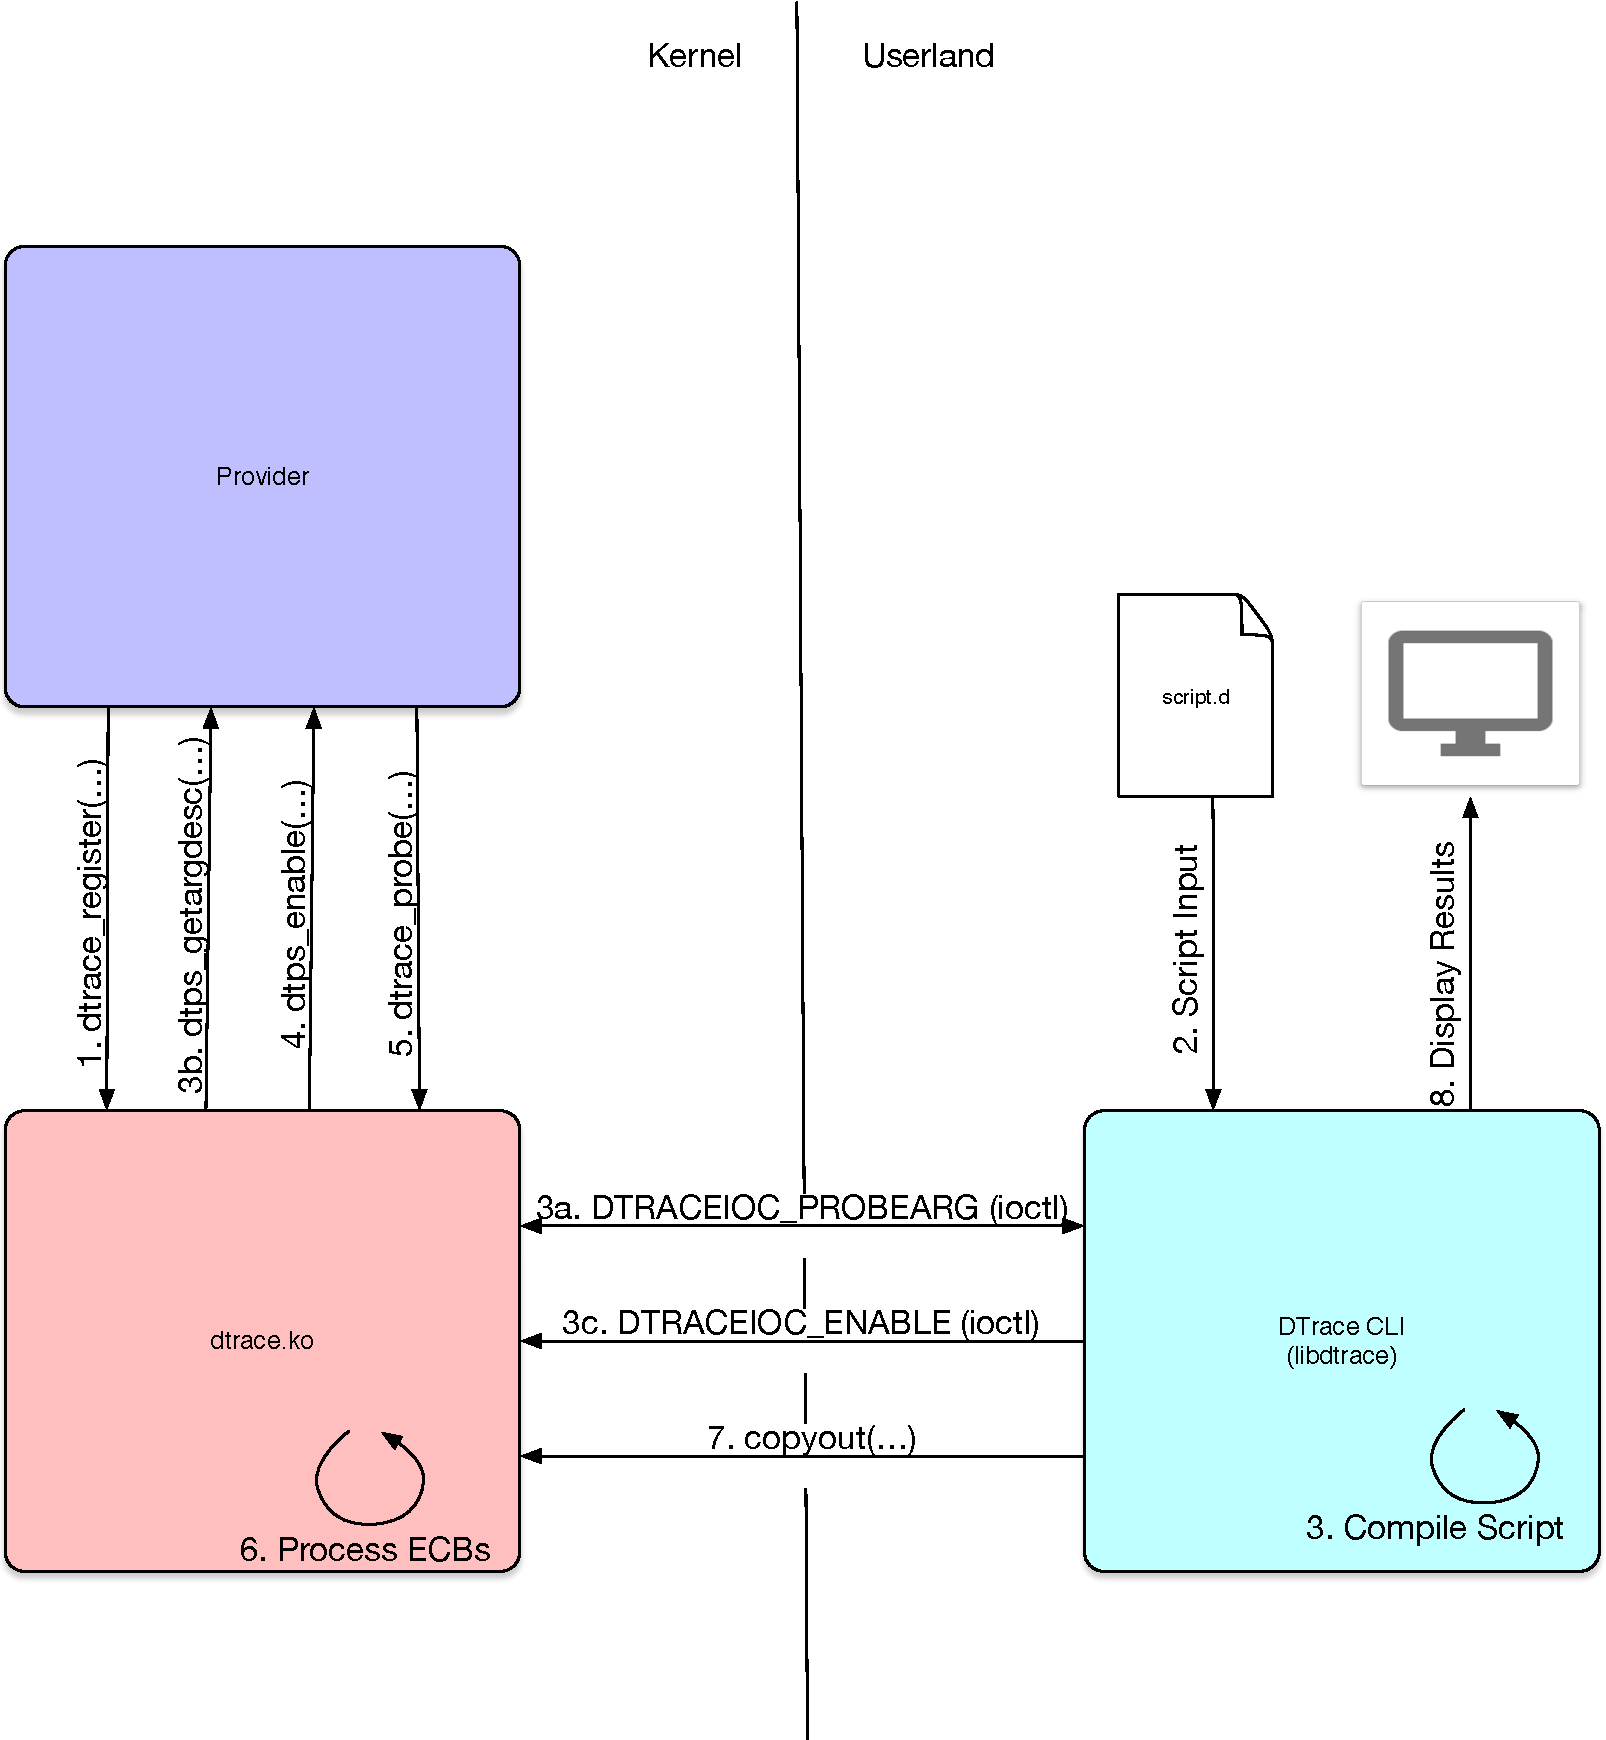
\includegraphics[width=0.8\linewidth]{dtrace-lifecycle.pdf}
	\caption{Lifecycle of an OpenDTrace Probe}
	\label{fig:lifecycle}
\end{figure}

When a provider is first loaded it registers itself with the
OpenDTrace kernel module (1). The registration process causes the
provider to enumerate all of its available probes, which are also
disabled by default.

The provider and kernel module remain idle until instrumentation is
requested. Instrumentation is requested via the \texttt{dtrace}
command in cooperation with the \texttt{libdtrace} library.  The the
user provides a D script, specifying the code to be run when a probe
fires (2). When the \texttt{dtrace} command executes it initializes
the \texttt{libdtrace} library, which in turn causes the kernel module
to initialize its tracing state and set up memory buffers to stored
the trace data.

The \texttt{libdtrace} library then compiles the D script (3). As part
of this process the compiler queries the kernel module to determine
the arguments for probes of interest via an ioctl (3a). The kernel in
turn queries the provider for a description of the probe arguments
which are returned to the compiler.  If the arguments discovered by
the kernel module do not match those supplied in the D script the
compiler will signal an error and abort compilation of the D script.
If the script did not supply any type information, the compilation
will complete and any mismatch will result in a runtime error.

The result of the D script compilation is a set of Enabling Control Blocks
(ECB)s.  An ECB is created for each enabling, or probe point, as well
as for each action statement in a D language clause.
The ECBs are provided to the kernel module (3c) which stores them,
with others, in a tree like structure. Once an ECB is safely stored in
the kernel, the kernel module tells the provider to enable the probes
that are to be instrumented.

Enabling a probe means telling the provider that at the right point
the \verb|dtrace_probe| kernel function must be called.  All tracing
ultimately goes through the \verb|dtrace_probe| function in the
kernel, which is responsible for all of the work related to any part
of tracing.  How \verb|dtrace_probe| is ultimately called depends on
both the program and the provider.

The function boundary tracepoint (\verb|fbt|) and \verb|fasttrap|
providers which allow tracing of kernel code and user space code,
respectively, both operate under the same model.  They both find the
instruction in the program at which the tracepoint is to be placed and
swap the regular instruction with a an architecture dependent
break-point instruction when tracing is enabled.

The profile provider is completely different from the FBT or fasttrap
providers as it is meant to call \verb|dtrace_probe| on a periodic
basis using in-kernel timers.  Enabling a profile provider does not
change any instruction stream in any program, but instead adds calls
to \verb|dtrace_probe| to the kernel's timing machinery.

When code execution reaches a point that has an enabled probe, the
probe fires and a call is made into the kernel module (5). The kernel
module then walks through the tree of ECBs, executing any that match
the probe that was fired (6). The captured data is written into the
buffer created when \texttt{libdtrace} was initialized. At a later
point the data is copied out of the kernel by the library (7), and
then the final results are made available to the end user (8).

\section{Trace Records}
\label{sec:trace-records}

When tracing is enabled the OpenDTrace modules in the kernel produce a
stream of records which are consumed by the \verb|dtrace(1)| command
and turned into various types of output.  Records are communicated in
a buffer structure, \verb|dtrace_bufdata| which is shared between the
kernel and user space.  Buffers contain one of two types of data.
Either the data is a plain record, or it is an aggregation.  All data
is arranged as a stream of bytes where the current header gives the
extent of the data, indicating where the next record can be found.

Plain records contain the data requested by the D script along with
optional formatting information and arguments.  Aggregations are
treated specially because they are not simply raw data buffers, but
instead, contain information that descibes deltas, normalized data,
and information on data binning.

\section{Privilege Model}
\label{sec:privilege}

The OpenDTrace privilege model is relatively simple, any program that
wishes to trace another program, or the operating system kernel, must
be running with \emph{root} privileges.  Some operating systems, such
as Illumos, provide a more nuanced privilege model.

%%% Local Variables:
%%% mode: latex
%%% TeX-master: "dtrace-specification"
%%% End:
